\documentclass[landscape,final,a0paper,fontscale=0.285]{baposter}

\usepackage[vlined]{algorithm2e}
\usepackage{calc}
\usepackage{graphicx}
\usepackage{amsmath}
\usepackage{amssymb}
\usepackage{relsize}
\usepackage{multirow}
\usepackage{rotating}
\usepackage{bm}
\usepackage{url}
\usepackage{setspace}
\usepackage{wrapfig}
\usepackage{graphicx}
\usepackage{multicol}
\usepackage{pbox}
%\usepackage{times}
%\usepackage{helvet}
%\usepackage{bookman}
\usepackage{palatino}

\newcommand{\captionfont}{\footnotesize}

\graphicspath{{images/}{../images/}}
\usetikzlibrary{calc}

\newcommand{\SET}[1]  {\ensuremath{\mathcal{#1}}}
\newcommand{\MAT}[1]  {\ensuremath{\boldsymbol{#1}}}
\newcommand{\VEC}[1]  {\ensuremath{\boldsymbol{#1}}}
\newcommand{\Video}{\SET{V}}
\newcommand{\video}{\VEC{f}}
\newcommand{\track}{x}
\newcommand{\Track}{\SET T}
\newcommand{\LMs}{\SET L}
\newcommand{\lm}{l}
\newcommand{\PosE}{\SET P}
\newcommand{\posE}{\VEC p}
\newcommand{\negE}{\VEC n}
\newcommand{\NegE}{\SET N}
\newcommand{\Occluded}{\SET O}
\newcommand{\occluded}{o}

%%%%%%%%%%%%%%%%%%%%%%%%%%%%%%%%%%%%%%%%%%%%%%%%%%%%%%%%%%%%%%%%%%%%%%%%%%%%%%%%
%%%% Some math symbols used in the text
%%%%%%%%%%%%%%%%%%%%%%%%%%%%%%%%%%%%%%%%%%%%%%%%%%%%%%%%%%%%%%%%%%%%%%%%%%%%%%%%

%%%%%%%%%%%%%%%%%%%%%%%%%%%%%%%%%%%%%%%%%%%%%%%%%%%%%%%%%%%%%%%%%%%%%%%%%%%%%%%%
% Multicol Settings
%%%%%%%%%%%%%%%%%%%%%%%%%%%%%%%%%%%%%%%%%%%%%%%%%%%%%%%%%%%%%%%%%%%%%%%%%%%%%%%%
\setlength{\columnsep}{1.5em}
\setlength{\columnseprule}{0mm}

%%%%%%%%%%%%%%%%%%%%%%%%%%%%%%%%%%%%%%%%%%%%%%%%%%%%%%%%%%%%%%%%%%%%%%%%%%%%%%%%
% Save space in lists. Use this after the opening of the list
%%%%%%%%%%%%%%%%%%%%%%%%%%%%%%%%%%%%%%%%%%%%%%%%%%%%%%%%%%%%%%%%%%%%%%%%%%%%%%%%
\newcommand{\compresslist}{%
\setlength{\itemsep}{1pt}%
\setlength{\parskip}{0pt}%
\setlength{\parsep}{0pt}%
}

%%%%%%%%%%%%%%%%%%%%%%%%%%%%%%%%%%%%%%%%%%%%%%%%%%%%%%%%%%%%%%%%%%%%%%%%%%%%%%
%%% Begin of Document
%%%%%%%%%%%%%%%%%%%%%%%%%%%%%%%%%%%%%%%%%%%%%%%%%%%%%%%%%%%%%%%%%%%%%%%%%%%%%%

\begin{document}

%%%%%%%%%%%%%%%%%%%%%%%%%%%%%%%%%%%%%%%%%%%%%%%%%%%%%%%%%%%%%%%%%%%%%%%%%%%%%%
%%% Here starts the poster
%%%---------------------------------------------------------------------------
%%% Format it to your taste with the options
%%%%%%%%%%%%%%%%%%%%%%%%%%%%%%%%%%%%%%%%%%%%%%%%%%%%%%%%%%%%%%%%%%%%%%%%%%%%%%
% Define some colors

%\definecolor{lightblue}{cmyk}{0.83,0.24,0,0.12}
\definecolor{lightblue}{rgb}{0.145,0.6666,1}

% Draw a video
\newlength{\FSZ}
\newcommand{\drawvideo}[3]{% [0 0.25 0.5 0.75 1 1.25 1.5]
   \noindent\pgfmathsetlength{\FSZ}{\linewidth/#2}
   \begin{tikzpicture}[outer sep=0pt,inner sep=0pt,x=\FSZ,y=\FSZ]
   \draw[color=lightblue!50!black] (0,0) node[outer sep=0pt,inner sep=0pt,text width=\linewidth,minimum height=0] (video) {\noindent#3};
   \path [fill=lightblue!50!black,line width=0pt] 
     (video.north west) rectangle ([yshift=\FSZ] video.north east) 
    \foreach \x in {1,2,...,#2} {
      {[rounded corners=0.6] ($(video.north west)+(-0.7,0.8)+(\x,0)$) rectangle +(0.4,-0.6)}
    }
;
   \path [fill=lightblue!50!black,line width=0pt] 
     ([yshift=-1\FSZ] video.south west) rectangle (video.south east) 
    \foreach \x in {1,2,...,#2} {
      {[rounded corners=0.6] ($(video.south west)+(-0.7,-0.2)+(\x,0)$) rectangle +(0.4,-0.6)}
    }
;
   \foreach \x in {1,...,#1} {
     \draw[color=lightblue!50!black] ([xshift=\x\linewidth/#1] video.north west) -- ([xshift=\x\linewidth/#1] video.south west);
   }
   \foreach \x in {0,#1} {
     \draw[color=lightblue!50!black] ([xshift=\x\linewidth/#1,yshift=1\FSZ] video.north west) -- ([xshift=\x\linewidth/#1,yshift=-1\FSZ] video.south west);
   }
   \end{tikzpicture}
}

\hyphenation{resolution occlusions}
%%
\begin{poster}%
  % Poster Options
  {
  % Show grid to help with alignment
  grid=false,
  % Column spacing
  colspacing=0.5em,
  % Color style
  bgColorOne=white,
  bgColorTwo=white,
  borderColor=red,
  headerColorOne=black,
  headerColorTwo=red,
  headerFontColor=white,
  boxColorOne=white,
  boxColorTwo=lightblue,
  % Format of textbox
  textborder=roundedleft,
  % Format of text header
  eyecatcher=true,
  headerborder=closed,
  headerheight=0.13\textheight,
%  textfont=\sc, An example of changing the text font
  headershape=roundedright,
  headershade=shadelr,
  headerfont=\Large\bf\textsc, %Sans Serif
  textfont={\setlength{\parindent}{1.5em}},
  boxshade=plain,
%  background=shade-tb,
  background=plain,
  linewidth=1pt,
  columns=5
  }
  % Eye Catcher
  {\includegraphics[width=16em]{images/mcgill_logo}} 
  % Title
  {\bf\textsc{\larger An Efficient Fault-Tolerant Sensor Fusion \\ \vspace{0.2em} Algorithm for Accelerometers}\vspace{0.3em} }
  % Authors
  {\smaller \textsc{O. Sarbishei, B. Nahill, A. Roshan Fekr, M. Janidarmian, K. Radecka, Z. Zilic, B. Karajica \\
  {\footnotesize Department of Electrical \& Computer Engineering, McGill University, Montreal, Canada; ST Microelectronics}
  }}
  % University logo
  {\includegraphics[width=16em]{images/logo_iml_red}}

%\put(-15,545){\includegraphics[width=0.7\paperwidth,height=13em]{images/bg_top.pdf}}
%\reflectbox{
%\put(-963,545){\includegraphics[width=0.7\paperwidth,height=13em]{images/bg_top.pdf}}
%}

%%%%%%%%%%%%%%%%%%%%%%%%%%%%%%%%%%%%%%%%%%%%%%%%%%%%%%%%%%%%%%%%%%%%%%%%%%%%%%
%%% Now define the boxes that make up the poster
%%%---------------------------------------------------------------------------
%%% Each box has a name and can be placed absolutely or relatively.
%%% The only inconvenience is that you can only specify a relative position 
%%% towards an already declared box. So if you have a box attached to the 
%%% bottom, one to the top and a third one which should be in between, you 
%%% have to specify the top and bottom boxes before you specify the middle 
%%% box.
%%%%%%%%%%%%%%%%%%%%%%%%%%%%%%%%%%%%%%%%%%%%%%%%%%%%%%%%%%%%%%%%%%%%%%%%%%%%%%
    %
    % A coloured circle useful as a bullet with an adjustably strong filling
    \newcommand{\colouredcircle}{%
      \tikz{\useasboundingbox (-0.2em,-0.32em) rectangle(0.2em,0.32em); \draw[draw=black,fill=lightblue,line width=0.03em] (0,0) circle(0.18em);}}


%%%%%%%%%%%%%%%%%%%%%%%%%%%%%%%%%%%%%%%%%%%%%%%%%%%%%%%%%%%%%%%%%%%%%%%%%%%%%%
\headerbox{Motivations}{name=motivations,column=0,span=4,row=0}{
%%%%%%%%%%%%%%%%%%%%%%%%%%%%%%%%%%%%%%%%%%%%%%%%%%%%%%%%%%%%%%%%%%%%%%%%%%%%%%
\begin{multicols}{3}
{\sc Continuous Glucose Monitor (CGM) sensors inaccurate, yet part of critical systems where accuracy and reliability are of utmost importance}
\vspace{-0.5em}
\begin{itemize} \compresslist
\item Require frequent calibration due to deterioration, changes in position, and other factors
\item Interest in multi-CGM fusion and fault tolerance for improved accuracy and resiliency -- Take many sensors to produce a single \emph{best} estimate, accounting for risk of sensor failure
\item Needs to be tolerant of multiple faults, provide quick response, and be efficient for use in wearable, power-constrained systems
\item \textbf{Problem:} Study and experimentation requires complex experimental setup
\item Until we can develop experimental platform, we can explore other sensor types
\end{itemize}
\pagebreak

\noindent
\begin{minipage}{\columnwidth}
	{\sc Temperature sensors and accelerometers experience similar problems and many applications demand high-accuracy, fault-tolerant sensor readings}
	\begin{itemize} \compresslist
	\item More accessible reference than CGM means we can perform experiments to gather data
	\item Test against known reference stimuli to demonstrate fusion and fault-tolerant methods
	\end{itemize}
\end{minipage}


\end{multicols}
}


%%%%%%%%%%%%%%%%%%%%%%%%%%%%%%%%%%%%%%%%%%%%%%%%%%%%%%%%%%%%%%%%%%%%%%%%%%%%%%
\headerbox{Temperature Sensor Experimentation}{name=temp-experimentation,
           column=0,span=2,below=motivations}{
%%%%%%%%%%%%%%%%%%%%%%%%%%%%%%%%%%%%%%%%%%%%%%%%%%%%%%%%%%%%%%%%%%%%%%%%%%%%%%
\begin{multicols}{2}
\noindent
\begin{minipage}[b][6.8cm][t]{\columnwidth+0.5\columnsep}
	\begin{wrapfigure}{r}{0.5\columnwidth}
	\vspace{-1em}
	\includegraphics[width=0.5\columnwidth]{tp4500}
	\vspace{-2em}
	\end{wrapfigure}
	We developed a system of 8 STTS751 temperature sensors to log readings in a Temptronic TP4500 controlled temperature chamber for a reference~\cite{atena:iccd}.
	\begin{itemize} \compresslist
		\item Use 8 STTS751 digital temperature sensors in TP4500 temperature control chamber
		\item Gather over 100,000 samples at $4^\circ$C intervals from $10^\circ$C to $30^\circ$C to calibrate and characterize sensor error for use in fusion and fault-detection
	\end{itemize}
\end{minipage}

\noindent
\begin{minipage}[t][6.8cm][t]{\columnwidth}
	\begin{center}
		\includegraphics[width=\columnwidth]{temp_err_dist}
		\vspace{-0.2em}
		{\sc Gaussian fitting of sensor errors}
	\end{center}
	
	\begin{itemize}\compresslist
		\item Calibration produces zero-mean distributions fitted to Gaussian
		\item Use individual sensor statistics for fault detection thresholds and weighting in fusion.
	\end{itemize}
\end{minipage}

%\begin{center}
%\includegraphics[width=0.8\columnwidth]{tp4500}
%\includegraphics[width=0.8\columnwidth]{temp_calib}
%\end{center}

\end{multicols}

}

\headerbox{Accelerometer Experimentation}{name=acc-experimentation,
           column=2,span=2,below=motivations,bottomaligned=temp-experimentation}{
%%%%%%%%%%%%%%%%%%%%%%%%%%%%%%%%%%%%%%%%%%%%%%%%%%%%%%%%%%%%%%%%%%%%%%%%%%%%%%
\begin{multicols}{2}


\noindent
\begin{minipage}{\columnwidth}
	\begin{wrapfigure}{r}{0.4\columnwidth}
	\vspace{-1em}
	\includegraphics[width=0.4\columnwidth]{acc_setup}
	\vspace{-2em}
	\end{wrapfigure}
	
	\indent We designed an experiment with 5 MMA8451Q digital accelerometers at 800Hz on a track using a 1200FPS camera as a reference for speed. 
	
	Prior off-line calibration with over 30,000 reference samples is performed with all sensors mounted to account for discrepancies in manufacturing and mounting. Coefficients are generated using the linear least-squares method~\cite{st:calib}.
\end{minipage}

\noindent
\begin{minipage}{\columnwidth}
	\begin{wrapfigure}{l}{0.55\columnwidth}
		\vspace{-1em}
		\begin{center}
			\includegraphics[width=0.6\columnwidth]{acc_reference}
		\end{center}
		\vspace{-2em}
	\end{wrapfigure}

	New fault screening technique demonstrated greatly improved MSE in fault conditions compared with previous work. \\
	
	\begin{minipage}{\columnwidth}
		\noindent \begin{tabular}{|c|c|c|c|}
		\hline
			\multirow{2}{*}{\pbox{20cm}{\# Faulty \\ Sensors}} & \multicolumn{3}{|c|}{MSE} \\
		\cline{2-4}
			& M1 \cite{zilic:wh} & M2 \cite{atena:iccd} & \textbf{M3} \\
		\hline
			0 & \multicolumn{3}{|c|}{\textbf{0.6199}} \\
		\hline
			1 & 0.8414 & \multicolumn{2}{|c|}{\textbf{0.802}} \\
		\hline
			2 & 5.112 & 5.1449 & \textbf{1.8778} \\
		\hline
		\end{tabular}
	\end{minipage}
\end{minipage}

\end{multicols}

}



%%%%%%%%%%%%%%%%%%%%%%%%%%%%%%%%%%%%%%%%%%%%%%%%%%%%%%%%%%%%%%%%%%%%%%%%%%%%%%
\headerbox{References}{name=references,column=0,
                       below=temp-experimentation,above=bottom}{
%%%%%%%%%%%%%%%%%%%%%%%%%%%%%%%%%%%%%%%%%%%%%%%%%%%%%%%%%%%%%%%%%%%%%%%%%%%%%%
\smaller
\bibliographystyle{ieee}
\renewcommand{\section}[2]{\vskip 0.05em}
\begin{thebibliography}{1}\itemsep=-0.01em
	\setlength{\baselineskip}{0.4em}
	
	\bibitem{atena:iccd}
	A.~Roshan~fekr, M.~Janidarmian, O.~Sarbishei, B.~Nahill, K.~Radecka, Z.~Zilic,
	\newblock{``MSE Minimization and Fault-Tolerant Data Fusion for Multi-Sensor Systems''},
	\newblock{\em IEEE ICCD},
	\newblock{Oct. 2012, pp. 445-452.}

	\bibitem{zilic:wh}
	Z.~Zilic, K.~Radecka,
	\newblock{``Fault Tolerant Glucose Sensor Readout and Recalibration,''}
	\newblock{Proceedings of Wireless Health, WH, 2011}

	\bibitem{st:calib}
	STMicroelectronics. \newblock (2010, Apr.).
	\newblock{\em Tilt Measurement Using a Low-g 3-Axis Accelerometer},
	\newblock{\em Application Note AN3182 [Online]}
%      \bibitem{awf:tracking}
%        A.~Buchanan and A.~Fitzgibbon.
%        \newblock {I}nteractive {F}eature {T}racking using {K-D} {T}rees and {D}ynamic {P}rogramming.
%        \newblock In {\em CVPR '06}
\end{thebibliography}
\vspace{4em}
}
%%%%%%%%%%%%%%%%%%%%%%%%%%%%%%%%%%%%%%%%%%%%%%%%%%%%%%%%%%%%%%%%%%%%%%%%%%%%%%
\headerbox{Future Developments}{name=future,column=1,span=3,
                                aligned=references,above=bottom}{
%%%%%%%%%%%%%%%%%%%%%%%%%%%%%%%%%%%%%%%%%%%%%%%%%%%%%%%%%%%%%%%%%%%%%%%%%%%%%%
\begin{center}
{\large \bf
Multiple paths to expand on our findings:
\vspace{-0.8em}
}
\end{center}
\begin{multicols}{2}

\noindent
\begin{minipage}{\columnwidth+\columnsep}
	\begin{center}
	\textsc{Hybrid in-silico/in-vitro CGM experimental setup}
	\end{center}
	\begin{center}
	\vspace{-1.2em}
	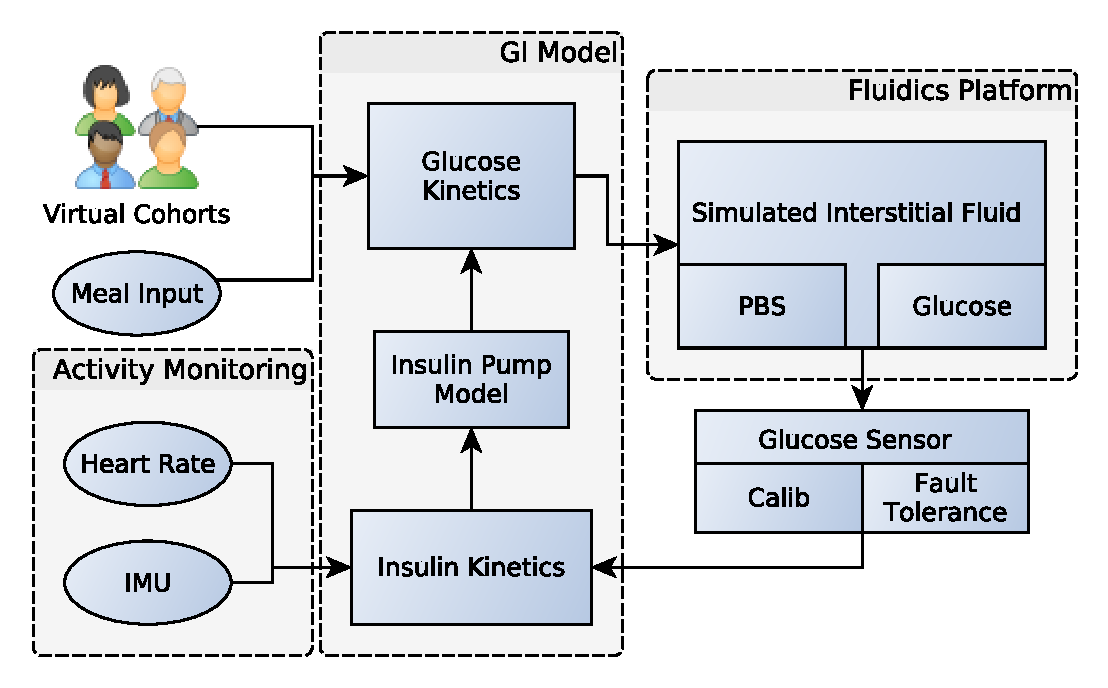
\includegraphics[width=0.78\textwidth]{CLIC}
	\end{center}
	
	\vspace{-1.8em}
	
	Allow for the substitution of models, hardware, and experimental algorithms anywhere in the loop
\end{minipage}

\pagebreak

\noindent
\begin{minipage}{\columnwidth}
	\begin{center}
	\textsc{Explore further and more elaborate applications of fault-tolerant fusion in inertial sensors}
	\vspace{0em}
	\end{center}
	
	{\sc Limitations of proposed technique:} Restricted to linear-motion case where sensor readings are identical
	
	\vspace{0.5em}
	
	{\sc More practical extension:} Use spatially distributed accelerometers augmented with gyroscopes and/or magnetometers as well to compensate for rotation
	\vspace{-0.5em}
	\begin{itemize} \compresslist
	\item Derive fault-tolerance from direct redundancy and that of spatially-separated accelerometer pair and gyroscope
	\end{itemize}
\end{minipage}


\end{multicols}
\vspace{0.3em}
}


%%%%%%%%%%%%%%%%%%%%%%%%%%%%%%%%%%%%%%%%%%%%%%%%%%%%%%%%%%%%%%%%%%%%%%%%%%%%%%
\headerbox{Fusion Process}{name=fusion-process,column=4,span=1,row=0,bottomaligned=motivations}{
%%%%%%%%%%%%%%%%%%%%%%%%%%%%%%%%%%%%%%%%%%%%%%%%%%%%%%%%%%%%%%%%%%%%%%%%%%%%%%
Propose three-step procedure for fault-tolerant data fusion:
\vspace{-0.7em}
\begin{enumerate}\compresslist
	\item Offline fixed-position calibration against reference (gravity)
	\item Sensor fault screening
	\item Fusion of non-faulty sensor data
\end{enumerate}
\vspace{-0.7em}
The result is a minimum-MSE linear fusion with bounded maximum mismatch in fault conditions.
}



\headerbox{Fault Screening}{name=fault,column=4,span=1,below=fusion-process,bottomaligned=acc-experimentation}{
\begin{algorithm}[H]
	\linesnumbered
	\dontprintsemicolon
	\SetKwComment{Comment}{// }{}
	\KwData{$x_{1:n}$; {\em // $n$ sensor readings}}
	\KwData{$M_{1:n}$; {\em // Max sensor deviation}}
	\For{m {\bf in} 1:n}{
		\nl $sum = \sum_{j=1}^{n}x_j$\;
		\nl
		\For{i {\bf in} 1:n}{
			\nl $a_i=\frac{sum-x_i}{n-1}$\;
			\nl $d_i=\left| x_i - a_i \right|$\;
		}
		\For{i {\bf in} 1:n}{
			\If{$d_i = \max{d_{1:n}}$}{
				\nl break\;
			}
			\If{$d_i > M_i$}{
				\nl Throw away $x_i$\;
				\nl $n = n - 1$\;
			}
		}
		\nl return $x_{1:n}$ \;
	}
\end{algorithm}
}


%%%%%%%%%%%%%%%%%%%%%%%%%%%%%%%%%%%%%%%%%%%%%%%%%%%%%%%%%%%%%%%%%%%%%%%%%%%%%%
  \headerbox{Minimum-MSE Fusion}{name=fusion,column=4,span=1,below=fault,above=bottom}{
%%%%%%%%%%%%%%%%%%%%%%%%%%%%%%%%%%%%%%%%%%%%%%%%%%%%%%%%%%%%%%%%%%%%%%%%%%%%%%
\noindent Linear fusion: $\displaystyle x_{est}=\sum_{j=1}^{n}c_j x_j$ \\
\vspace{-0.3em}
%For an error function independent of $x_{ref}$, \\
%\vspace{-0.5em}
\begin{align*}
x_{ref}(1-\sum_{j=1}^{n}c_j)=0 \Longrightarrow \sum_{j=1}^{n}c_j = 1
\end{align*}
\vspace{-0.8em}
Optimal coefficients are \\
\vspace{-0.8em}
\begin{align*}
c_j = \frac{1}{S_j \sum_{k=1}^{n}\frac{1}{S_k}}
\end{align*}

where $S_j$ is the average square error for sensor $j$. For zero-mean error (calibrated), this is the noise variance.
}





\end{poster}

\end{document}
